\documentclass[12pt,a4paper]{article}
\usepackage[utf8]{inputenc}
\usepackage[T2A]{fontenc}
\usepackage[english,russian]{babel}
\usepackage{amsmath}
\usepackage{booktabs}
\usepackage{float}
\usepackage{geometry}
\usepackage{graphicx}
\usepackage{hyperref}
\usepackage{indentfirst}
\usepackage{listings}
\usepackage{verbatim}

\geometry{left=25mm,right=15mm,top=20mm,bottom=20mm}

\lstset{
  basicstyle=\ttfamily\small,
  breaklines=true,
  columns=fullflexible,
  frame=single,
  keepspaces=true,
  showstringspaces=false,
  tabsize=4
}

\newcommand{\StudentName}{Д.\,А.~Скрылев}
\newcommand{\StudentCourse}{1}
\newcommand{\StudentGroup}{2ИВТ}
\newcommand{\SupervisorName}{С.\,В.~Теплоухов}
\newcommand{\ReportCity}{Майкоп}
\newcommand{\ReportYear}{2026}

\begin{document}
\pagenumbering{gobble}

\begin{titlepage}
\begin{center}
\large
МИНИСТЕРСТВО НАУКИ И ВЫСШЕГО ОБРАЗОВАНИЯ РОССИЙСКОЙ ФЕДЕРАЦИИ

Федеральное государственное бюджетное образовательное учреждение высшего образования

\textbf{АДЫГЕЙСКИЙ ГОСУДАРСТВЕННЫЙ УНИВЕРСИТЕТ}

\vspace{0.25cm}

НОК ``Институт точных наук и цифровых технологий''

Кафедра автоматизированных систем обработки информации и управления

\vfill

\textsc{Отчет по практике}\\[5mm]

{\LARGE Лабораторная работа №2}\\[3mm]
{\Large Решение системы линейных алгебраических уравнений методом простой итерации}

\vfill

Вариант №1

Точность вычислений: \(\varepsilon = 0.01\)

\StudentCourse{} курс, группа \StudentGroup

\vfill

\begin{flushright}
\begin{minipage}{0.45\textwidth}
Выполнил:\\
\underline{\hspace{2cm}} \StudentName\\[4mm]
Руководитель:\\
\underline{\hspace{2cm}} \SupervisorName
\end{minipage}
\end{flushright}

\vfill

\ReportCity, \ReportYear{} г.
\end{center}
\end{titlepage}

\pagenumbering{arabic}
\tableofcontents
\newpage

\section{Постановка задачи}

Необходимо решить систему линейных алгебраических уравнений
\[
AX = B
\]
с точностью \(\varepsilon = 0.01\). По варианту №1 используется метод простой итерации.

Исходные данные:
\[
A =
\begin{pmatrix}
5 & 0 & 1\\
1 & 3 & -1\\
-3 & 2 & 10
\end{pmatrix},
\qquad
B =
\begin{pmatrix}
11\\
4\\
6
\end{pmatrix}.
\]

Контрольный ответ:
\[
X \approx
\begin{pmatrix}
2\\
1\\
1
\end{pmatrix}.
\]

\section{Теоретические сведения}

Система линейных алгебраических уравнений \(AX=B\) состоит из матрицы коэффициентов \(A\), вектора неизвестных \(X\) и вектора свободных членов \(B\). Решением системы является такой вектор \(X\), при подстановке которого все уравнения системы выполняются.

Метод простой итерации относится к численным методам. Система приводится к виду
\[
X^{(n+1)} = C X^{(n)} + d,
\]
где \(C\) --- матрица итераций, \(d\) --- вектор свободных членов итерационного процесса, \(n\) --- номер итерации.

Начальное приближение в работе выбрано равным
\[
X^{(0)} =
\begin{pmatrix}
0\\
0\\
0
\end{pmatrix}.
\]

Если норма матрицы итераций \(q=\|C\|_{\infty}\) меньше единицы, то итерационный процесс сходится. Для контроля точности используется апостериорная оценка:
\[
R_n = \frac{q}{1-q}\left\|X^{(n)}-X^{(n-1)}\right\|_{\infty}.
\]
Вычисления прекращаются при выполнении условия
\[
R_n \leq \varepsilon.
\]

\section{Проверка сходимости}

Для данной системы выполняется строгое диагональное преобладание по строкам:
\[
|5| > |0| + |1|,
\qquad
|3| > |1| + |-1|,
\qquad
|10| > |-3| + |2|.
\]

Следовательно, система подходит для применения метода простой итерации, а итерационный процесс должен сходиться.

\section{Переход к итерационному виду}

Исходная система имеет вид:
\[
\begin{cases}
5x_1 + x_3 = 11,\\
x_1 + 3x_2 - x_3 = 4,\\
-3x_1 + 2x_2 + 10x_3 = 6.
\end{cases}
\]

Выразим каждую переменную через остальные:
\[
\begin{cases}
x_1 = \dfrac{11 - x_3}{5},\\[2mm]
x_2 = \dfrac{4 - x_1 + x_3}{3},\\[2mm]
x_3 = \dfrac{6 + 3x_1 - 2x_2}{10}.
\end{cases}
\]

Итерационные формулы:
\[
\begin{cases}
x_1^{(n+1)} = \dfrac{11 - x_3^{(n)}}{5},\\[2mm]
x_2^{(n+1)} = \dfrac{4 - x_1^{(n)} + x_3^{(n)}}{3},\\[2mm]
x_3^{(n+1)} = \dfrac{6 + 3x_1^{(n)} - 2x_2^{(n)}}{10}.
\end{cases}
\]

В матричном виде:
\[
C =
\begin{pmatrix}
0 & 0 & -0.2\\
-\frac{1}{3} & 0 & \frac{1}{3}\\
0.3 & -0.2 & 0
\end{pmatrix},
\qquad
d =
\begin{pmatrix}
2.2\\
\frac{4}{3}\\
0.6
\end{pmatrix}.
\]

Норма матрицы итераций:
\[
\|C\|_{\infty} =
\max(0.2,\;0.666667,\;0.5) = 0.666667 < 1.
\]
Это подтверждает сходимость метода.

\section{Программа}

Программа написана на языке Python. Она хранит матрицу \(A\) и вектор \(B\), проверяет диагональное преобладание, строит итерационную матрицу \(C\), выполняет итерации до достижения заданной точности, выводит таблицу итераций и проверяет невязку \(AX-B\).

\subsection{Основной фрагмент исходного кода}

Полный исходный код программы находится в файле \texttt{main.py}. Ниже приведен основной фрагмент, отвечающий за построение итерационной системы и выполнение метода простой итерации.

\begin{lstlisting}[language=Python]
EPSILON = 0.01
A = (
    (5.0, 0.0, 1.0),
    (1.0, 3.0, -1.0),
    (-3.0, 2.0, 10.0),
)
B = (11.0, 4.0, 6.0)
X0 = (0.0, 0.0, 0.0)


def build_iteration_system(matrix, vector):
    c_rows = []
    d_values = []

    for i, row in enumerate(matrix):
        diagonal = row[i]
        c_row = []

        for j, value in enumerate(row):
            c_row.append(0.0 if i == j else -value / diagonal)

        c_rows.append(tuple(c_row))
        d_values.append(vector[i] / diagonal)

    return tuple(c_rows), tuple(d_values)


def matrix_vector_product(matrix, vector):
    return tuple(
        sum(value * vector[j] for j, value in enumerate(row))
        for row in matrix
    )


def simple_iteration(matrix, vector, initial, epsilon):
    c_matrix, d_vector = build_iteration_system(matrix, vector)
    q = max(sum(abs(value) for value in row) for row in c_matrix)
    previous = initial
    rows = []

    for n in range(1, 101):
        product = matrix_vector_product(c_matrix, previous)
        current = tuple(product[i] + d_vector[i] for i in range(len(product)))
        delta = max(abs(current[i] - previous[i]) for i in range(len(current)))
        error_estimate = q / (1.0 - q) * delta
        rows.append((n, current, delta, error_estimate))

        if error_estimate <= epsilon:
            return current, rows

        previous = current

    raise RuntimeError("Simple iteration did not converge.")
\end{lstlisting}

\section{Таблица итераций}

В таблице обозначено:
\[
\Delta_n = \left\|X^{(n)}-X^{(n-1)}\right\|_{\infty},
\qquad
R_n = \frac{q}{1-q}\Delta_n.
\]

\begin{table}[H]
\centering
\caption{Таблица итераций метода простой итерации}
\small
\begin{tabular}{rrrrrr}
\toprule
$n$ & $x_1$ & $x_2$ & $x_3$ & $\Delta_n$ & $R_n$ \\
\midrule
1 & 2.200000 & 1.333333 & 0.600000 & 2.200000 & 4.400000 \\
2 & 2.080000 & 0.800000 & 0.993333 & 0.533333 & 1.066667 \\
3 & 2.001333 & 0.971111 & 1.064000 & 0.171111 & 0.342222 \\
4 & 1.987200 & 1.020889 & 1.006178 & 0.057822 & 0.115644 \\
5 & 1.998764 & 1.006326 & 0.991982 & 0.014563 & 0.029126 \\
6 & 2.001604 & 0.997739 & 0.998364 & 0.008587 & 0.017173 \\
7 & 2.000327 & 0.998920 & 1.000933 & 0.002569 & 0.005138 \\
\bottomrule
\end{tabular}
\normalsize
\end{table}


На последней итерации \(R_n \leq 0.01\), поэтому требуемая точность достигнута.

\section{Скриншот запуска программы}

\begin{figure}[H]
\centering
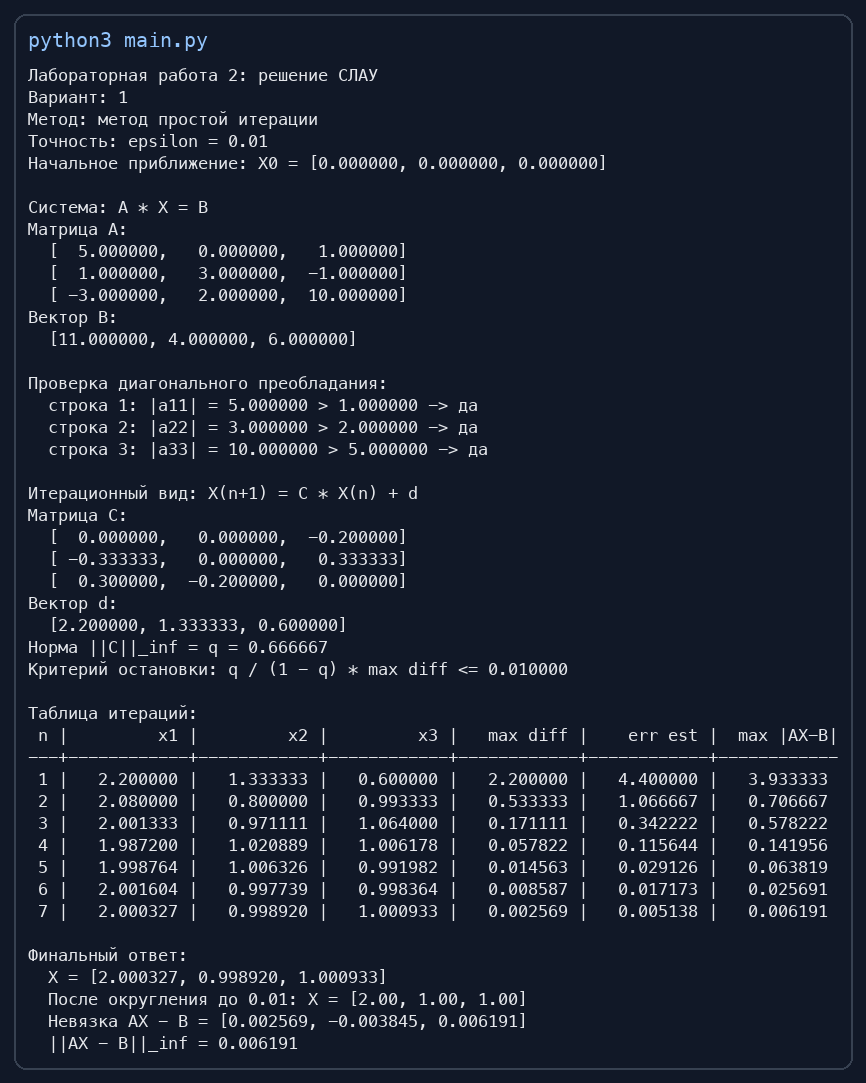
\includegraphics[width=0.98\textwidth]{assets/program_output.png}
\caption{Результат запуска программы}
\end{figure}

\section{Результаты}

После выполнения итераций получен вектор:
\[
X \approx
\begin{pmatrix}
2.000327\\
0.998920\\
1.000933
\end{pmatrix}.
\]

После округления до сотых:
\[
X \approx
\begin{pmatrix}
2.00\\
1.00\\
1.00
\end{pmatrix}.
\]

Невязка для найденного приближенного решения:
\[
AX - B \approx
\begin{pmatrix}
0.002569\\
-0.003845\\
0.006191
\end{pmatrix},
\qquad
\|AX-B\|_{\infty} \approx 0.006191.
\]

Контрольная проверка для точного округленного ответа:
\[
A
\begin{pmatrix}
2\\
1\\
1
\end{pmatrix}
=
\begin{pmatrix}
11\\
4\\
6
\end{pmatrix}
= B.
\]

\section{Вывод}

В ходе лабораторной работы была решена система линейных алгебраических уравнений методом простой итерации. Проверка диагонального преобладания и норма матрицы итераций подтвердили сходимость метода. Полученное приближенное решение совпадает с контрольным ответом после округления:
\[
X \approx (2.00;\;1.00;\;1.00).
\]
Требуемая точность \(\varepsilon = 0.01\) достигнута.

\end{document}
